\documentclass[10pt,a4paper]{article}
\usepackage[T1]{fontenc}
\usepackage[utf8]{inputenc}
\usepackage{lmodern,microtype}
\usepackage[margin=22mm,headheight=14pt]{geometry}
\usepackage{graphicx,booktabs,longtable,array,ragged2e,pdflscape}
\usepackage{xcolor}
\usepackage{caption,subcaption}
\usepackage{amsmath,amssymb}
\usepackage{seqsplit}
\usepackage{fancyhdr}
\usepackage[hidelinks]{hyperref}
\usepackage{url}
\definecolor{navy}{HTML}{24547A}
\hypersetup{colorlinks=true,linkcolor=navy,urlcolor=navy,citecolor=navy}
\urlstyle{tt}
\setlength{\parskip}{4pt}
\setlength{\parindent}{0pt}
\captionsetup{font=small,labelfont=bf}
\pagestyle{fancy}
\fancyhf{}
\fancyhead[L]{\small NumStability benchmark | ten-task evidence report}
\fancyhead[R]{\small 28 September 2026}
\fancyfoot[C]{\thepage}
\newcommand{\src}[1]{\textsuperscript{\cite{#1}}}
\newcommand{\fig}[2]{%
\begin{figure}[p]\centering
\includegraphics[width=.96\textwidth]{figures/#1.pdf}
\caption{#2 All task values are derived from the sealed N/L pairs by the
reproducible ten-task plotting script.\cite{taskledger,plotcode}}
\end{figure}}
\newcommand{\heatfig}[2]{%
\begin{figure}[p]\centering
\includegraphics[width=.96\textwidth]{figures/#1.pdf}
\caption{#2 All task values are derived from the sealed N/L pairs by the
reproducible ten-task plotting script.\cite{taskledger,plotcode}}
\end{figure}\clearpage}
\newcommand{\compactfig}[2]{%
\begin{figure}[p]\centering
\includegraphics[width=.78\textwidth]{figures/#1.pdf}
\caption{#2 All task values are derived from the sealed N/L pairs by the
reproducible ten-task plotting script.\cite{taskledger,plotcode}}
\end{figure}}
\title{\vspace{-13mm}\textbf{NumStability in AI-Assisted Lean Formalization and Proof}\\[2mm]
\large A reproducible, exploratory ten-task N/L benchmark report}
\author{HighamBench evidence report}
\date{28 September 2026}
\begin{document}
\maketitle

\begin{abstract}
We compare a Mathlib-only condition (N) with the same Lean environment plus a
frozen NumStability library and one task-neutral orientation conversation (L).
All ten reported paper tasks ended with an audited faithful statement and a
zero-hole, kernel-accepted proof in both conditions. Across these pairs, L
used 19.7\% fewer nonblank proof-code lines (2,537 versus 3,158) and 22.5\%
less contestant-active time (5,410 versus 6,979 seconds), while using 34.7\%
more net-new tokens (1.716 versus 1.273 million). Charging the one-time L
scout once leaves a 19.9\% time advantage and 41.7\% token excess. The
formalization stage was 7.3\% slower for L; the proof stage was 29.9\% faster.
At realized-reuse scores 1, 2, and 3, aggregate time gains were $-9.1\%$,
$+19.3\%$, and $+31.1\%$. These are descriptive development results, not a
held-out causal estimate: task selection was outcome-informed, five tasks had
previously favorable results, and the reuse rubric was annotated after
outcomes. The five newly screened tasks alone used 6.4\% more L proof lines.
\src{summary,selection,reuse}
\end{abstract}

\section{Question, corpus, and scientific status}

The question is whether a numerical-stability library reduces the work and
Lean code needed for an AI formalizer to state \emph{and prove} selected paper
results. Both conditions receive the same hashed source paper, task packet,
Lean 4, Mathlib, formalization prompt, audit policy, and proof requirement. L
alone receives frozen NumStability source and compiled declarations plus an
orientation appendix. Neither condition receives a shared Lean theorem
scaffold encoding the desired result.\src{protocol,prompts,taskledger}

The ten analyzed tasks span five source clusters: three Castaldo--Whaley--
Chronopoulos dot-product tasks, four Blanchard--Higham--Higham
log-sum-exp/softmax tasks, and one each from Hallman--Ipsen, Higham, and Rump.
Four tasks were marked hard in the frozen task metadata. The corpus is not a
random sample of numerical stability: tasks were selected for expected
library relevance, and the final reported ten were chosen after outcome
review. Five were previously favorable both-proved tasks. This is therefore
an \emph{outcome-informed exploratory development corpus}, not a prospective
or held-out evaluation. The dated selection manifest is public, while the
figures and numeric discussion here use only the ten reported tasks.
\src{selection,source,taskledger}

The measured result combines sealed pairs from two campaign identities. One
audit-schema incident required a new, separately identified pair; the valid
sealed pairs were not rerun. A pre-contestant deployment-index incident is
preserved separately and is not a measured task outcome. The public pair
archives retain prompts, candidate hashes, audit decisions, accepted Lean
files, proof checks, and hardware records. The ten-task derived ledger
preserves original pair identities and source SHA-256 values.\src{taskledger,evidence,recovery}

\begin{table}[ht]\centering\small
\begin{tabular}{@{}llrl@{}}\toprule
Cluster & Source & Tasks & PDF SHA-256 prefix\\\midrule
CAST08 & Castaldo et al., superblock dot product & 3 & \texttt{ffdea8e2136c7f42}\\
H20 & Higham, \emph{Accuracy and Stability}, Problem 20.8 & 1 & \texttt{7ca85d5caf3ffd5a}\\
HI21 & Hallman--Ipsen, summation-tree bounds & 1 & \texttt{cce25923a86d5d20}\\
P14 & Blanchard et al., log-sum-exp/softmax & 4 & \texttt{7247047bc49218e0}\\
RUMP12 & Rump, summation/dot-product error & 1 & \texttt{4b23ffc2f7588ddc}\\
\bottomrule\end{tabular}
\caption{Five paper/source clusters. Selected task-packet and PDF hashes are
in \texttt{generated/source\_registry.json}.\cite{registry,packets}}
\label{tab:papers}
\end{table}

\section{Frozen protocol and execution}

\subsection{Two stages, two clocks, and an independent audit}

A contestant first submits a Lean theorem with a single allowed
\texttt{sorry} occupying its target proof. There are at most four frozen
statement submissions. Each is hashed before off-clock compilation,
integrity validation, and independent candidate-specific faithfulness audit.
An unfaithful statement receives condition-neutral feedback in the same
formalizer conversation. Once a faithful statement is frozen, the model gets
up to four submissions to prove that \emph{exact proposition}. A proof with
\texttt{sorry}, \texttt{admit}, changed dependencies, extra axioms, or a trust
escape is not accepted. Proof success requires zero-hole Lean validation.
The formalizer is explicitly told not to submit a partial proof as complete.
\src{protocol,prompts,taskledger}

\begin{figure}[ht]\centering\small
\fbox{\begin{minipage}{.91\linewidth}\centering
Identical hashed PDF + source packet + common prompt\\[2mm]
$\downarrow$\\[2mm]
N: Mathlib \quad|\quad L: Mathlib + NumStability + one-time scout\\[2mm]
$\downarrow$\\[2mm]
Timed statement turns (max four) $\rightarrow$ hash $\rightarrow$ off-clock compile and audit\\[2mm]
$\downarrow$ faithful statement frozen\\[2mm]
Timed proof turns (max four) $\rightarrow$ hash $\rightarrow$ off-clock kernel check\\[2mm]
$\downarrow$ paired record, logs, and direct-declaration scan
\end{minipage}}
\caption{Source-first workflow. Audit and validation cost is recorded but not
charged to contestant-active clocks.\cite{protocol,metrics}}
\label{fig:flow}
\end{figure}

Faithfulness is binary. A full-domain equivalent statement or accepted
strengthening may pass; a narrowing of the paper's domain does not. The audit
uses fresh, stateless and condition-blind blind-translation, direct,
round-trip, and adjudication roles with dependency-aware semantic material.
These agents are independent of the formalizers. A faithful statement is not
counted as a proof; the zero-hole proof gate is separate. Some accepted
statements are equivalent while others are strengthenings, which can affect
the proof effort even when both pass.\src{protocol,auditprompts,taskledger}

The formalizer was GPT-6 Sol at high reasoning effort in both conditions;
GPT-6 Astra/high performed auditing. Contestant subagents and multi-agent
tools were disabled and attested by session controls. Observable tool and
turn events were archived; hidden chain-of-thought was not available.
Access used ChatGPT sign-in through Codex CLI 0.156.0, not metered API
billing.\src{metrics,evidence,deployment}

\subsection{Prompts and library access}

The common prompt says the PDF is authoritative and asks for the paper's
full domain, quantifiers, operation order, rounding model, constants, and
conclusion. It warns of independent faithfulness review and later proof.
N receives this prompt with Mathlib. L receives the same prompt plus a short
appendix encouraging deliberate discovery of the relevant algorithm
representation, compatible floating-point model, and error/perturbation
lemmas. L has access to the full library, not an oracle or task-specific
retrieval packet. A separate strict no-hole proof prompt is frozen.\src{prompts,proofprompt}

\begin{table}[ht]\centering\small
\begin{tabular}{@{}ll@{}}\toprule
Prompt & SHA-256 prefix\\\midrule
Common statement & \texttt{c3ece6ddddf2b2c}\\
L treatment appendix & \texttt{579a68943cfb636}\\
Task-neutral scout & \texttt{f2517b44f0801c0}\\
Proof-stage base & \texttt{b21295790a3ff3f}\\
Strict no-hole proof prompt & \texttt{537ebad7810ec9a}\\
Audit roles & exact hashes in archived campaign inputs\\
\bottomrule\end{tabular}
\caption{Prompt identity; source files and observed effective prompts in the
archives provide full text.\cite{prompts,proofprompt,evidence}}
\end{table}

The task-neutral L scout ran once for 183.313 seconds using GPT-6 Sol/high.
It used 1,274,811 input tokens, 1,193,216 of them cached, plus 6,873 output
tokens: 88,468 net-new tokens by the benchmark formula. The provider total
including cached input was 1,281,684 tokens. Its frozen orientation root
was forked into task conversations; the scout was never rerun per task.
\src{warmroot,warmscout}

\subsection{Hardware, parallelism, and software}

Titan ran Linux/x86-64 on an Intel Core i9-13900K. Three disjoint lanes ran
concurrently, each capped at eight logical CPUs, 24~GiB RAM, zero swap, and
512 processes. N/L order alternated by frozen schedule index. CPU affinity,
cgroups, before/after machine snapshots, and sampled per-turn peaks were
logged. In the ten reported tasks, sampled per-condition maxima were 5.39
cores and 2.35~GiB for N, and 4.70 cores and 2.01~GiB for L. Brief spikes
could be missed. Parallelism reduced campaign makespan; it did not divide
individual contestant-active time.\src{summary,evidence}

Lean was \texttt{leanprover/lean4:v4.29.0-rc3}, Mathlib commit
\texttt{\seqsplit{e8ea1afc32790ce1d4e1a4e45cc412ba9388716b}}, and
NumStability commit
\texttt{\seqsplit{45813a95dacf577461bae13f033af0dbc985a225}}.
The separately recorded full-library build took 1,315.18 seconds after
Mathlib dependency-cache preparation; it is not charged to task-active time.
The build record identifies hardware, cache state, command, output digest,
and resource measurements. Authentication material and compiled caches are
not redistributed.\src{buildrecord,librarysnapshot,runtimesnapshot}

\section{Metrics and denominators}

Formalization time includes contestant-active work through the frozen
faithful statement, including ordinary library search and repairs. Proof
time starts after that statement is frozen and includes proof turns and
rejected submissions. Their sum is task-active time. Compilation, dossier
construction, and auditing are separately measured excluded overhead. The
headline time is neither whole campaign makespan nor end-to-end wall time.
Net-new tokens equal input minus cached input plus output; full provider
usage including cached input is retained separately. Code lines exclude
blank and comment-only lines. All ten pairs have faithful statements and
complete proofs in both conditions, so paired proof denominators are ten.
Warm-inclusive per-task panels allocate the one-time L scout evenly over ten
for visualization; aggregate and cumulative calculations charge it once.
Positive N-to-L gain means less L cost.\src{metrics,taskledger,warmroot}

\begin{table}[ht]\centering\small
\begin{tabular}{@{}lrrrr@{}}\toprule
Metric (ten tasks, summed) & N & L & L/N & L gain\\\midrule
Formalization seconds & 1,389.1 & 1,490.2 & 1.073 & -7.3\% \\
Proof seconds & 5,589.8 & 3,920.0 & 0.701 & +29.9\% \\
Total active seconds & 6,978.9 & 5,410.2 & 0.775 & +22.5\% \\
Total + warm seconds & 6,978.9 & 5,593.5 & 0.801 & +19.9\% \\
Formalization net-new tokens & 399,748 & 980,733 & 2.453 & -145.3\% \\
Proof net-new tokens & 873,571 & 734,899 & 0.841 & +15.9\% \\
Total net-new tokens & 1,273,319 & 1,715,632 & 1.347 & -34.7\% \\
Total + warm net-new tokens & 1,273,319 & 1,804,100 & 1.417 & -41.7\% \\
Statement code lines & 333 & 337 & 1.012 & -1.2\% \\
Proof code lines & 3,158 & 2,537 & 0.803 & +19.7\% \\
\bottomrule

\end{tabular}
\caption{Machine-generated aggregates. The one-time scout is charged once in
the two warm-inclusive rows.\cite{summary,plotcode}}
\label{tab:aggregate}
\end{table}

\section{Time, token, and code outcomes}

L was faster on eight of ten tasks and used fewer proof-code lines on six of
ten. Formalization cost 7.3\% more active time and 2.45 times as many net-new
tokens for L; proof used 29.9\% less time and 15.9\% fewer net-new tokens.
Mean time was 697.9 seconds/task for N and 541.0 for L, or 559.3 with the
scout allocated. Mean net-new tokens were 127.3 thousand for N and 171.6
thousand for L, or 180.4 thousand with the scout. The time and proof-line
gains do not imply token savings. Every task label in the figures carries
its realized-reuse score as \texttt{(R=x/3)}; aggregate plots print the score
distribution.\src{summary,reuse,plotcode}

\fig{01_total_time_ex_warm}{Per-task total contestant-active time, excluding the one-time scout. Task-time library search remains included.}
\fig{02_total_time_in_warm}{Per-task active time with $183.313/10=18.331$ warm seconds allocated to each L bar. This is one scout, not ten.}
\fig{03_phase_times}{Formalization and proof components of task-active time, excluding off-clock audit and validation.}
\fig{04_total_tokens_ex_warm}{Per-task net-new contestant tokens, excluding the warm scout and cached input.}
\fig{05_total_tokens_in_warm}{Per-task net-new tokens with $88{,}468/10=8{,}847$ scout tokens allocated to each L task.}
\fig{06_phase_tokens}{Formalization and proof net-new tokens; L's statement-stage cost is visible separately.}
\fig{07_averages}{Arithmetic means per task for time, tokens, and code; warm-inclusive bars allocate the scout over ten tasks.}
\fig{08_code_lines}{Final faithful statement and complete proof code lines, excluding blanks and comments.}

The one-time cost is best read cumulatively: it is paid before any task, not
as a repeated delay. Figure~\ref{fig:cumulative} shows that the active-time
advantage survives charging it once. The token deficit grows. Cached-prefix
processing is reported separately rather than being misrepresented as zero
resource use.\src{summary,warmroot}

\begin{figure}[p]\centering
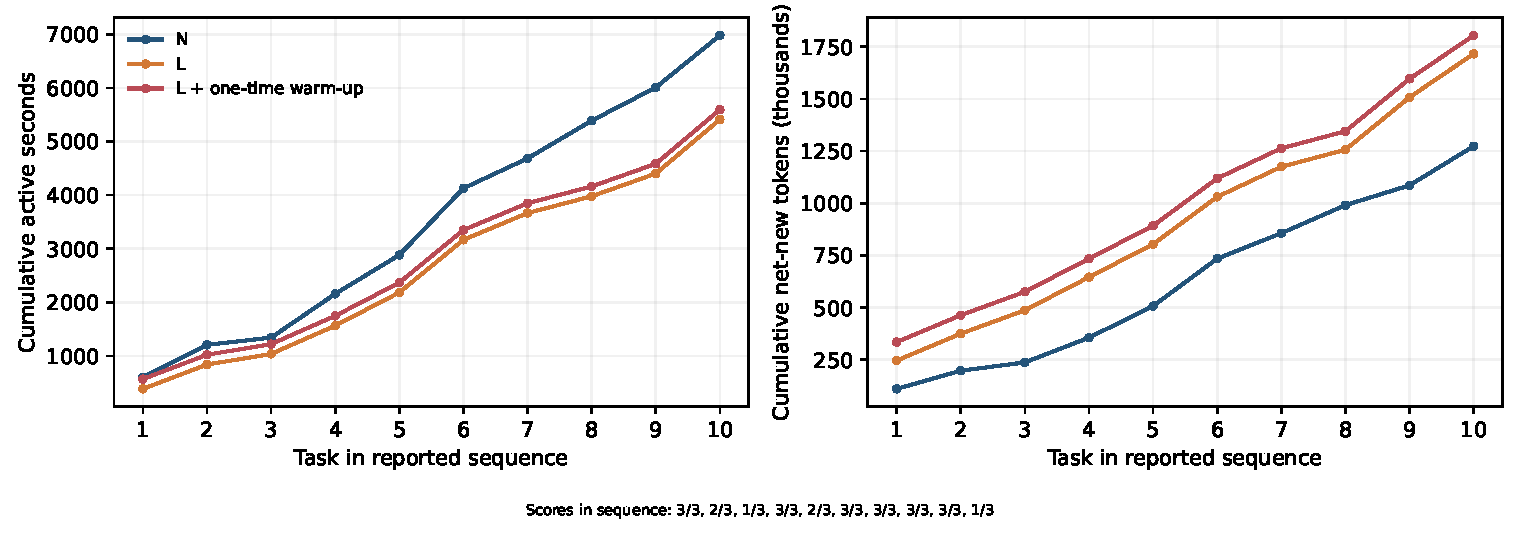
\includegraphics[width=.95\textwidth]{figures/12_cumulative_warm.pdf}
\caption{Cumulative contestant-active work in the ten-task order shown. The
red L curve charges the one-time scout once. This is not parallel campaign
makespan. Each score appears in the footer in plotted order.\cite{summary,plotcode}}
\label{fig:cumulative}\end{figure}

\section{Declaration uptake and overlap}

The declaration scan uses elaborated constants in final L statements and
kernel-accepted proof terms, including proof-local helper bodies. It is not
an import or text-match count. In the ten reported tasks, nine had
substantive NumStability statement reach, and all ten had direct proof-term
reach. Exact names, counts, and statement/proof surfaces are in the
machine-readable declaration and reuse ledgers.\src{declscan,reuse,taskledger}

The five score--gain heatmaps share one interpretation: the horizontal axis
is realized reuse score, the vertical axis is the named N-to-L gain in
percent, and darker cells contain more tasks. An occupied cell prints the
exact gain values of its tasks, even when two fall in the same fixed-width
bin. The empty score-zero column is shown rather than suppressed. Positive
gain means L used less time, fewer tokens, or fewer proof lines. These are
descriptive, binned views of ten observations, not fitted relationships.
Their exact bin edges and task memberships are published.\src{heatmapcells,reuse}

\heatfig{09a_reuse_formalization_gain}{Reuse score versus formalization-time gain. Each occupied cell prints exact task gains in percent; shade encodes the number of tasks.}
\heatfig{09b_reuse_proof_gain}{Reuse score versus proof-time gain, with the same cell convention.}
\heatfig{09c_reuse_total_gain}{Reuse score versus total contestant-active-time gain, excluding the one-time warm-up.}
\heatfig{09d_reuse_tokens_gain}{Reuse score versus total net-new-token gain. Negative values mean L used more tokens.}
\heatfig{09e_reuse_proof_lines_gain}{Reuse score versus proof-code-line gain, computed from final kernel-accepted proofs.}
\compactfig{10_direct_declaration_scatter}{Distinct direct proof-term NumStability names against time, token, proof-line, and formalization-time gains. White numerals are the reuse scores. Rank coefficients are descriptive at $n=10$.}

Within these ten, direct proof-name count has Spearman rank correlation
$\rho=+0.56$ with total-time gain and $\rho=+0.64$ with proof-line gain.
That is a descriptive association only: tasks were selected after outcomes,
the number of direct declarations can track proof complexity, and these
small-sample coefficients do not identify a causal effect of library
coverage. Formalization submissions vary little, so an attempt correlation
would be uninformative. Model search appears in archived events, but this
trial did not isolate a causal ``query overhead'' variable.\src{summary,evidence}

The five previously favorable tasks show 34.0\% less active time and 37.6\%
fewer proof lines for L. The five newly screened tasks show 7.2\% less active
time but 6.4\% \emph{more} proof lines. This split is essential: pooled code
gains are concentrated in the previously successful group. The cohort
chart keeps those identities visible without implying independent sampling.
\src{summary,selection}

\fig{11_cohort_strata}{Aggregate N-to-L time, proof-line, and token gains for the five previously favorable tasks, five newly screened tasks, and all ten reported tasks. Each panel includes the reuse-score distribution.}

\subsection{Source-task-specific realized reuse}

The three-role index counts (1) task-relevant numeric/FP/gamma/norm
\emph{foundation}, (2) computation or rounding \emph{interface}, and (3)
proved error/bound or mathematical \emph{analysis}. A role scores one only
if an exact witness appears in the final L statement or kernel-accepted
proof term; an analysis witness must appear in the proof. Imports,
text-only mentions, and transitive-only dependencies score zero. The score
is an ordinal 0--3 breadth index, not a count of modules or a proof-line
savings estimate. Every task obligation and exact witness is published.
\src{reusemap,reuse,declscan}

The rubric was written after outcomes were seen, not by a blind assessor.
It is validated against archived statement/proof names and task-packet
hashes but cannot turn realized use into prospective library coverage. Six
tasks score 3, two score 2, and two score 1. Aggregate active-time gains by
score are $-9.1\%$, $+19.3\%$, and $+31.1\%$; proof-line gains are
$-4.2\%$, $-1.2\%$, and $+31.4\%$. The pooled score--time rank association
is $\rho=+0.72$, while proof-line association is $\rho=+0.58$. For the five
newly screened tasks alone, the corresponding coefficients are $+0.63$ and
$-0.32$. These post-selection, tiny-group statistics must not be read as
confirmatory significance tests.\src{summary,reuse,selection}

The two gain--gain heatmaps put formalization against proof time, and total
active time against total net-new tokens. Both axes are N-to-L percentage
gains; zero lines separate improvement from regression. Cell shade gives the
mean reuse score of the task(s) in that bin, and cell text gives each task
number and its reuse score (R0--R3). The
task-number key is printed inside each figure and exact memberships are in
the heatmap ledger. Bins show coarse joint patterns; they do not create
additional observations.\src{heatmapcells,taskledger}

\heatfig{14a_formalization_vs_proof_gain}{Formalization-time gain versus proof-time gain. Task numbers and reuse scores appear in occupied cells; the upper-right quadrant means L was faster in both phases.}
\heatfig{14b_total_time_vs_tokens_gain}{Total active-time gain versus total net-new-token gain. The upper-right quadrant means L was faster and used fewer net-new tokens.}
\fig{15_reuse_score_groups}{Aggregate gains within displayed score 1, 2, and 3 groups, with sample counts. Code-size improvement is substantial only in score 3; tokens are unfavorable in every score stratum.}
\fig{16_attempts}{Frozen statement and proof submissions per task and condition, with the reuse score beside every task. Each stage allowed at most four submissions.}

Concrete examples show reusable material: CAST08-FIXED3 used dot-product
and recursive-sum interfaces, reducing proof code from 325 to 221 lines;
CAST08-PROP3.1 used summation/error declarations and reduced 373 to 200;
H20-8 used least-squares backward-error interfaces and reduced 243 to 167.
There are exceptions even at score 3: P14-LOGSUMEXP was faster but its L
proof had 257 versus 204 N lines. The score records observed breadth, not
what would have happened without the library.\src{taskledger,reuse,declscan}

\section{Audit overhead, hardware, and limitations}

The faithfulness audit was not a shortcut. Across the reported task records,
excluded audit role calls summed to 3,287 seconds and 3.23 million reported
tokens for N, and 3,625 seconds and 3.48 million for L. These are sums of
role calls, not contestant time or necessarily serial campaign wall time.
Compilation, semantic dossiers, and proof validation have separately logged
fields. Task formalization and proof stages consumed 27.26 million
provider-reported tokens including cached input for N and 55.06 million for
L; net-new tokens are the narrower primary comparison.\src{summary,taskledger}

\begin{figure}[p]\centering
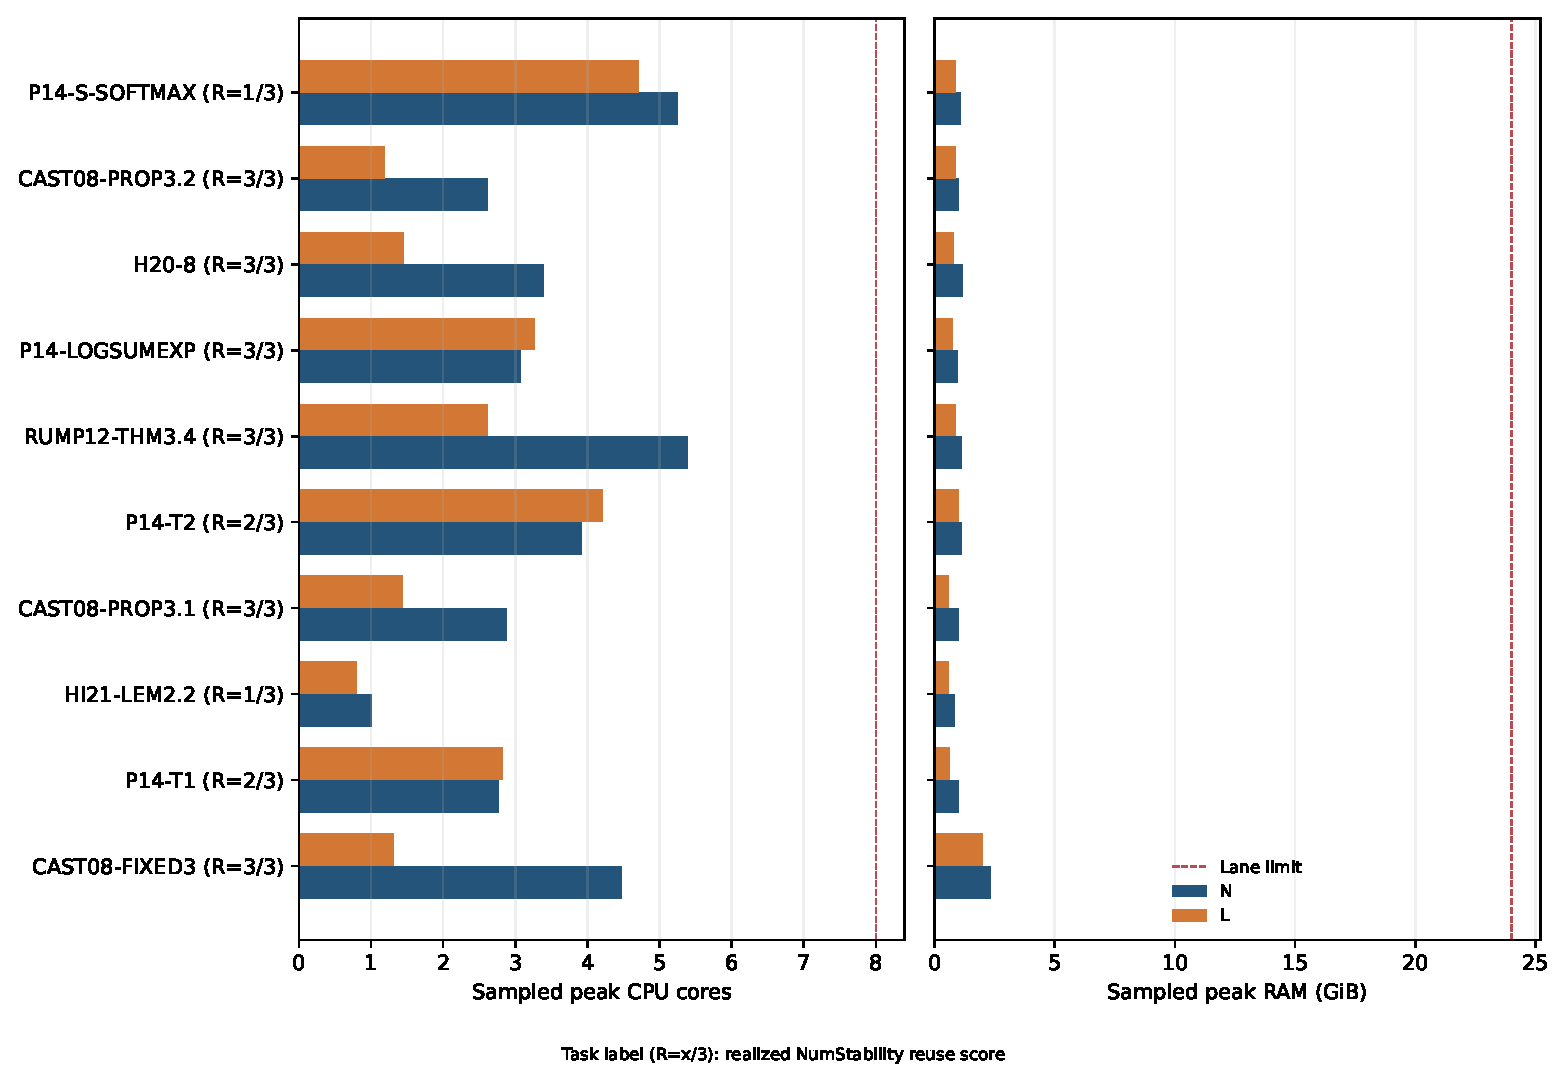
\includegraphics[width=.92\textwidth]{figures/13_hardware_peaks.pdf}
\caption{Sampled per-task CPU and RAM peaks against lane caps; brief
unobserved spikes are possible. Every task label includes the reuse score.
\cite{summary,taskledger}}
\end{figure}

Limitations include outcome-informed selection, five previously favorable
tasks, four related tasks from one paper, one run per task, no randomization,
an audit-schema incident with disclosed recovery, possible equivalent versus
stronger accepted statements, and dependence on a changing model service
for any future rerun. Warm L knowledge is a measured task-neutral scout,
not an actual fine-tuned model. Observed reuse does not isolate the causal
value of each declaration or prove that expansion of NumStability alone
would remove search, representation, or interface friction.
\src{selection,taskledger,protocol}

The strongest defensible conclusion is specific: in this ten-task,
outcome-informed development corpus, NumStability supplied directly used
components and L produced shorter and faster complete proofs in aggregate.
The highest realized-reuse group had the largest pooled proof-line and time
gains, but the new-only code result and token cost temper any general
coverage-benefit claim. Independent validation would require a task set and
reuse rubric fixed \emph{before} outcomes are observed.\src{summary,reuse}

\section{Reproducibility and source trail}

This branch provides the report source, plotting program, all generated
ten-task tables and figures, task ledger, reuse witnesses, declaration scan,
selected paper-source registry, dated selection manifest, frozen protocol,
prompts, controller sources, warm-scout record, and measured-pair evidence
archives. The script verifies ten exact task identities, paired success,
direct score witnesses, and source-input hashes. The repository verifier
checks the underlying sealed pair identities and sums. Source papers,
authenticated Codex state, and large compiled caches are not repackaged;
the source registry provides PDF hashes and task-packet identities. A rerun
can follow the pinned protocol but cannot guarantee bit-for-bit identical
model behavior.\src{readme,summary,registry,evidence}

Rebuild with the pinned Python requirements, then compile this
\texttt{report.tex} using \texttt{latexmk}. All displayed aggregate rows
and task-level appendices are generated from the derived ten-task ledger;
figures use unrounded values. The selected evidence is read-only: changing
any task, prompt, or library snapshot would require a new benchmark identity
rather than an edit to these results.\src{plotcode,readme,taskledger}

\clearpage
\appendix
\begin{landscape}
\section{Task-level numeric ledger}

The tables below contain only the ten reported tasks in their scheduled
order. Formalization and proof times are contestant-active seconds; token
totals are net-new thousands. SS means substantive statement-declaration
count and PT means direct proof-term declaration count. AF/AP are L
formalization/proof submission counts. All exact-precision values and both
conditions' attempt counts are in the machine-readable ledger.
\src{taskledger,plotcode}

\small
\begin{longtable}{@{}lrrrrrrrr@{}}
\caption{Task-level time and net-new token comparison, excluding warm-up.
\cite{taskledger,plotcode}}\label{tab:times}\\
\toprule Task & F-N & F-L & P-N & P-L & Total-N & Total-L & Tok-N(k) & Tok-L(k)\\\midrule\endfirsthead
\toprule Task & F-N & F-L & P-N & P-L & Total-N & Total-L & Tok-N(k) & Tok-L(k)\\\midrule\endhead
CAST08-FIXED3 & 123 & 112 & 481 & 275 & 603 & 387 & 111 & 246 \\
P14-T1 & 176 & 171 & 428 & 282 & 604 & 453 & 87 & 129 \\
HI21-LEM2.2 & 106 & 161 & 29 & 37 & 135 & 199 & 40 & 112 \\
CAST08-PROP3.1 & 170 & 180 & 646 & 347 & 816 & 527 & 119 & 159 \\
P14-T2 & 135 & 135 & 590 & 485 & 725 & 619 & 151 & 158 \\
RUMP12-THM3.4 & 156 & 230 & 1087 & 752 & 1243 & 982 & 227 & 227 \\
P14-LOGSUMEXP & 130 & 93 & 428 & 407 & 558 & 499 & 122 & 144 \\
H20-8 & 91 & 102 & 612 & 211 & 703 & 313 & 134 & 82 \\
CAST08-PROP3.2 & 155 & 124 & 464 & 300 & 619 & 423 & 95 & 251 \\
P14-SHIFTED-SOFTMAX & 148 & 183 & 823 & 826 & 972 & 1009 & 188 & 208 \\

\end{longtable}
\vspace{3mm}
\begin{longtable}{@{}llcrrrrrrrr@{}}
\caption{Final code size, declaration reach, and L submission counts.
\cite{taskledger,declscan,plotcode}}\label{tab:code}\\
\toprule Task & Cluster & Prior & Stmt-N & Stmt-L & Proof-N & Proof-L & SS & PT & AF & AP\\\midrule\endfirsthead
\toprule Task & Cluster & Prior & Stmt-N & Stmt-L & Proof-N & Proof-L & SS & PT & AF & AP\\\midrule\endhead
CAST08-FIXED3 & CAST08 & yes & 44 & 39 & 325 & 221 & 2 & 9 & 1 & 1 \\
P14-T1 & P14 & no & 27 & 29 & 201 & 227 & 2 & 7 & 1 & 1 \\
HI21-LEM2.2 & HI21 & no & 26 & 36 & 39 & 49 & 4 & 4 & 1 & 1 \\
CAST08-PROP3.1 & CAST08 & yes & 40 & 39 & 373 & 200 & 1 & 9 & 1 & 1 \\
P14-T2 & P14 & no & 35 & 37 & 364 & 345 & 0 & 13 & 1 & 1 \\
RUMP12-THM3.4 & RUMP12 & yes & 31 & 27 & 599 & 333 & 7 & 39 & 1 & 1 \\
P14-LOGSUMEXP & P14 & no & 28 & 27 & 204 & 257 & 2 & 8 & 1 & 1 \\
H20-8 & H20 & yes & 25 & 20 & 243 & 167 & 5 & 26 & 1 & 1 \\
CAST08-PROP3.2 & CAST08 & yes & 37 & 36 & 329 & 245 & 2 & 11 & 1 & 1 \\
P14-SHIFTED-SOFTMAX & P14 & no & 40 & 47 & 481 & 493 & 1 & 3 & 1 & 1 \\

\end{longtable}
\end{landscape}

\begin{landscape}
\section{Realized-reuse task ledger}

F, C, and A are foundation, computation/interface, and analysis roles. A
``yes'' means at least one exact witness was reached in the final L
statement or proof. The JSON ledger gives every witness and surface.
Positive gains favor L.\src{reusemap,reuse}

\small
\begin{longtable}{@{}lrcccrrrr@{}}
\caption{Realized-reuse breadth and paired N-to-L gains (percent).
\cite{reuse,plotcode}}\label{tab:reuse}\\
\toprule Task & Score & F & C & A & Proof lines & Proof time & Total time & Total tokens\\\midrule\endfirsthead
\toprule Task & Score & F & C & A & Proof lines & Proof time & Total time & Total tokens\\\midrule\endhead
CAST08-FIXED3 & 3 & yes & yes & yes & +32 & +43 & +36 & -123 \\
P14-T1 & 2 & yes & yes & -- & -13 & +34 & +25 & -48 \\
HI21-LEM2.2 & 1 & -- & yes & -- & -26 & -27 & -47 & -183 \\
CAST08-PROP3.1 & 3 & yes & yes & yes & +46 & +46 & +35 & -34 \\
P14-T2 & 2 & yes & -- & yes & +5 & +18 & +15 & -4 \\
RUMP12-THM3.4 & 3 & yes & yes & yes & +44 & +31 & +21 & +0 \\
P14-LOGSUMEXP & 3 & yes & yes & yes & -26 & +5 & +10 & -18 \\
H20-8 & 3 & yes & yes & yes & +31 & +66 & +56 & +39 \\
CAST08-PROP3.2 & 3 & yes & yes & yes & +26 & +35 & +32 & -164 \\
P14-SHIFTED-SOFTMAX & 1 & yes & -- & -- & -2 & -0 & -4 & -11 \\

\end{longtable}
\end{landscape}

\section{Direct declaration-usage index}

Family labels are descriptive; the JSON declaration scan contains exact
elaborated names in statements and proof terms. Imports and text-only
mentions are not counted.\src{declscan,taskledger}

\small
\begin{longtable}{@{}p{.22\textwidth}p{.27\textwidth}rp{.3\textwidth}r@{}}
\caption{Substantive statement and direct proof-term declaration families.
\cite{declscan,plotcode}}\\
\toprule Task & Statement family & $n$ & Proof family & $n$\\\midrule\endfirsthead
\toprule Task & Statement family & $n$ & Proof family & $n$\\\midrule\endhead
CAST08-FIXED3 & recursive sum, dot product & 2 & recursive sum, dot product, gamma bound & 9 \\
P14-T1 & recursive sum & 2 & recursive sum & 7 \\
HI21-LEM2.2 & sum tree & 4 & sum tree & 4 \\
CAST08-PROP3.1 & recursive sum & 1 & recursive sum, gamma bound & 9 \\
P14-T2 & none & 0 & gamma bound, product error & 13 \\
RUMP12-THM3.4 & finite FP format & 7 & finite FP format & 39 \\
P14-LOGSUMEXP & recursive sum & 2 & recursive sum, gamma bound & 8 \\
H20-8 & least squares & 5 & least squares & 26 \\
CAST08-PROP3.2 & recursive sum & 2 & recursive sum, gamma bound & 11 \\
P14-SHIFTED-SOFTMAX & infinity norm & 1 & infinity norm & 3 \\

\end{longtable}
\normalsize

\section{Source registry and immutable identities}

Every figure and numerical table derives from the ten-task ledger and
summary. Method claims are linked to the frozen protocol, prompts, campaign
records, hardware snapshots, or proof evidence. The source-selection
manifest is retained for auditability; its outcome-informed status is part
of the study record.\src{summary,selection,readme}

\begin{longtable}{@{}p{.22\textwidth}>{\RaggedRight\arraybackslash}p{.7\textwidth}@{}}
\toprule Source & Path / identity\\\midrule\endfirsthead
\toprule Source & Path / identity\\\midrule\endhead
Ten-task ledger & \path{ten_task_report/generated/source_task_ledger.json}; its metadata records the sealed-result SHA-256.\\
Selected source registry & \path{ten_task_report/generated/source_registry.json}; task packets and paper-PDF hashes.\\
Warm scout & \path{thesis_report/evidence/warm-root.json}; SHA-256 begins \texttt{3401426d25ee278c}.\\
Direct declarations & \path{ten_task_report/generated/declaration_scan.json}; exact elaborated names.\\
Realized reuse & \path{ten_task_report/generated/realized_reuse.json}; task obligations and exact proof/statement witnesses.\\
Heatmap cells & \path{ten_task_report/generated/heatmap_cells.json}; bin edges, occupied cells, exact tasks and gain values.\\
Aggregate metrics & \path{ten_task_report/generated/summary.json}; all ten-task sums, score groups, source digests, and overhead.\\
Selection disclosure & \path{thesis_report/posthoc_10/generated/summary.json}; dated, outcome-informed selection manifest.\\
Measured pair evidence & Compressed Pilot 34/35 archives under \path{paper_bencmark/thesis_report/evidence/}; archive SHA-256 values in companion README.\\
Library build & \path{thesis_report/evidence/library-build-record.json}; SHA-256 begins \texttt{6f4581380982e51f}.\\
Runtime snapshot & \path{thesis_report/evidence/runtime-snapshot.json}; SHA-256 begins \texttt{9fac78511309a591}.\\
\bottomrule
\end{longtable}

\clearpage
\begin{thebibliography}{99}\footnotesize\RaggedRight\setlength{\itemsep}{0pt}\setlength{\parskip}{0pt}
\bibitem{summary} This report's generated ten-task summary, \path{paper_bencmark/thesis_report/ten_task_report/generated/summary.json}.
\bibitem{taskledger} Selected sealed task records, \path{paper_bencmark/thesis_report/ten_task_report/generated/source_task_ledger.json}; source result digest in metadata.
\bibitem{plotcode} Reproducible figure/table script, \path{paper_bencmark/thesis_report/ten_task_report/make_figures.py}.
\bibitem{selection} Dated post-outcome task-selection manifest, \path{paper_bencmark/thesis_report/posthoc_10/generated/summary.json}.
\bibitem{registry} Selected task packet and paper-source identities, \path{paper_bencmark/thesis_report/ten_task_report/generated/source_registry.json}.
\bibitem{source} Paper/source descriptions and task packets in \path{paper_bencmark/formalization_benchmark/design33/packets/}.
\bibitem{packets} Hash-frozen task packets in \path{paper_bencmark/formalization_benchmark/design33/packets/}; selected hashes in the source registry.
\bibitem{protocol} Proof-required source-first protocol, \path{paper_bencmark/formalization_benchmark/design27/PROTOCOL.md}.
\bibitem{metrics} Prospective metric contract, \path{paper_bencmark/formalization_benchmark/design33/METRICS.md}.
\bibitem{prompts} Frozen common formalization prompt and L appendix, \path{paper_bencmark/formalization_benchmark/design27/prompts/}.
\bibitem{proofprompt} Strict proof prompt, \path{paper_bencmark/prospective_proof_no_holes/PROOF_PROMPT.md}.
\bibitem{auditprompts} Faithfulness-audit role prompts, \path{paper_bencmark/formalization_benchmark/audit/prompts/}; effective prompt hashes in campaign input records.
\bibitem{warmroot} Frozen task-neutral warm-root record, \path{paper_bencmark/thesis_report/evidence/warm-root.json}.
\bibitem{warmscout} Scout prompt and observable transcript, \path{paper_bencmark/thesis_report/evidence/warm-scout/}.
\bibitem{evidence} Archived measured-pair prompts, candidates, audits, validators, hardware and final Lean files under \path{paper_bencmark/thesis_report/evidence/}; checksums in the companion README.
\bibitem{recovery} Archived campaign incident and recovery manifests in \path{paper_bencmark/pilot35/} and the measured-pair evidence archives.
\bibitem{deployment} Frozen campaign runtime and Codex CLI identity, archived campaign inputs in the evidence bundle.
\bibitem{buildrecord} NumStability full build record, \path{paper_bencmark/thesis_report/evidence/library-build-record.json}.
\bibitem{librarysnapshot} Library snapshot, \path{paper_bencmark/thesis_report/evidence/library-snapshot.json}.
\bibitem{runtimesnapshot} Runtime snapshot, \path{paper_bencmark/thesis_report/evidence/runtime-snapshot.json}.
\bibitem{declscan} This report's direct declaration ledger, \path{paper_bencmark/thesis_report/ten_task_report/generated/declaration_scan.json}.
\bibitem{reusemap} Source-task-specific, post-outcome three-role rubric, \path{paper_bencmark/thesis_report/reuse_obligations.json}.
\bibitem{reuse} This report's exact-witness reuse ledger, \path{paper_bencmark/thesis_report/ten_task_report/generated/realized_reuse.json}.
\bibitem{heatmapcells} Exact bin edges and task memberships for the seven gain heatmaps, \path{paper_bencmark/thesis_report/ten_task_report/generated/heatmap_cells.json}.
\bibitem{readme} Rebuild and source instructions, \path{paper_bencmark/thesis_report/ten_task_report/README.md}.
\end{thebibliography}
\end{document}
